\clearpage
\section{实现细节}
本节提供所提方法和实验的更多实现细节。

\subsection{训练设置}
在表 \ref{table:training_setting_main} 中，提供了 BEVFormer v2 在 \cref{table:sota_nuscenes} 中用于 InternImage-B~\cite{InternImage} 和 InternImage-XL 骨干网络的超参数和训练方案。

\let\ck\checkmark

\setlength{\tabcolsep}{5pt}
\setlength{\doublerulesep}{2\arrayrulewidth}
\renewcommand{\arraystretch}{1.0}
\begin{table}[ht]
    \caption{BEVFormer v2 使用 InternImage 骨干网络（Backbone）的主要结果训练设置。}
    \label{table:training_setting_main}
    \centering
    \begin{tabular}{l|cc}
        %\toprule
        backbone & InternImage-B & InternImage-XL \\
        \hline
        training epochs & 24 & 24 \\
        batch size & 16 & 32 \\
        optimizer & AdamW & AdamW \\
        base learning rate & 4e-4 & 5e-4 \\
        weight decay & 0.01 & 0.01 \\
        lr schedule & step decay & step decay\\
        layer-wise lr decay & 0.96 & 0.94 \\
        warmup iters & 2000 & 2000  \\
        warmup schedule & linear & linear \\
        gradient clip & 35 & 35 \\
        \hline
        image size & 640 $\times$ 1600 & 640 $\times$ 1600 \\
        IDA & \ck & \ck \\
        temporal interval & 4 seconds & 4 seconds \\
        bi-directional & \ck & \ck \\
        \hline
    \end{tabular}
    
\end{table}

在表 \ref{table:large_backbone} 中，本文还在其他骨干网络上构建了 BEVFormer v2 检测器，包括 ResNet-50~\cite{ResNet}、DLA-34~\cite{DLA}、ResNet-101~\cite{ResNet} 和 VoVNet-99~\cite{Vovnet}。其训练设置列于表 \ref{table:training_setting_other}。

\let\ck\checkmark

\setlength{\tabcolsep}{5pt}
\setlength{\doublerulesep}{2\arrayrulewidth}
\renewcommand{\arraystretch}{1.0}
\begin{table}[ht]
    \caption{BEVFormer v2 使用其他骨干网络（Backbone）的训练设置。}
    \label{table:training_setting_other}
    \centering
    \begin{tabular}{l|cccc}
        %\toprule
        backbone & R50 & DLA34 & R101 & V2-99 \\
        \hline
        batch size & \multicolumn{4}{c}{16} \\
        optimizer & \multicolumn{4}{c}{AdamW} \\
        base lr & \multicolumn{4}{c}{4e-4} \\
        backbone lr & 2e-4 & 2e-4 & 4e-5 & 4e-5 \\
        weight decay & \multicolumn{4}{c}{0.01} \\
        \hline
    \end{tabular}
    
\end{table}

\subsection{网络架构}
在 BEVFormer v2 中，图像骨干网络产生步长为8、16和32的3层特征图。本文在骨干网络后采用FPN（特征金字塔网络）\cite{FPN} 生成步长为8、16、32、64和128的5层特征。透视头使用全部5层特征，而BEV头使用前4层（步长为8、16、32和64）。

\noindent\textbf{透视头.} 本文采用 DD3D~\cite{DD3D} 实现的单阶段无锚框（Anchor-free）单目3D检测器，包含三个独立头：分类头（Classification Head）、2D检测头（2D Detection Head）和3D检测头（3D Detection Head）。
分类头生成每个物体类别的 logit。
2D头通过特征位置到边界的4个偏移量生成与类别无关的边界框，并产生2D中心度（Center-ness）。
2D检测损失 $\mathcal{L}_{2D}$ 源自 FCOS~\cite{fcos}。
3D头预测3D边界框，包含以下系数：异体朝向（Allocentric Orientation）的旋转角、框中心深度、特征位置到投影框中心的偏移量，以及相对于类别典型尺寸的尺寸偏差。
此外，3D头生成预测3D框相对于2D置信度的置信度。
它采用 \cite{MonoDIS} 中的解耦 L1 损失（Disentangled L1 Loss）用于3D边界框回归，以及自监督损失（Self-supervised Loss）用于3D置信度，分别记为 $\mathcal{L}_{3D}$ 和 $\mathcal{L}_{conf}$。
BEVFormer v2 的透视损失是2D检测损失、3D回归损失和3D置信度损失之和：
\begin{equation}
    \mathcal{L}_{pers} = \mathcal{L}_{2D} + \mathcal{L}_{3D} + \mathcal{L}_{conf}
\end{equation}
透视检测头的更多细节请参见 \cite{DD3D}。

\begin{figure*}[t]
    \centering
    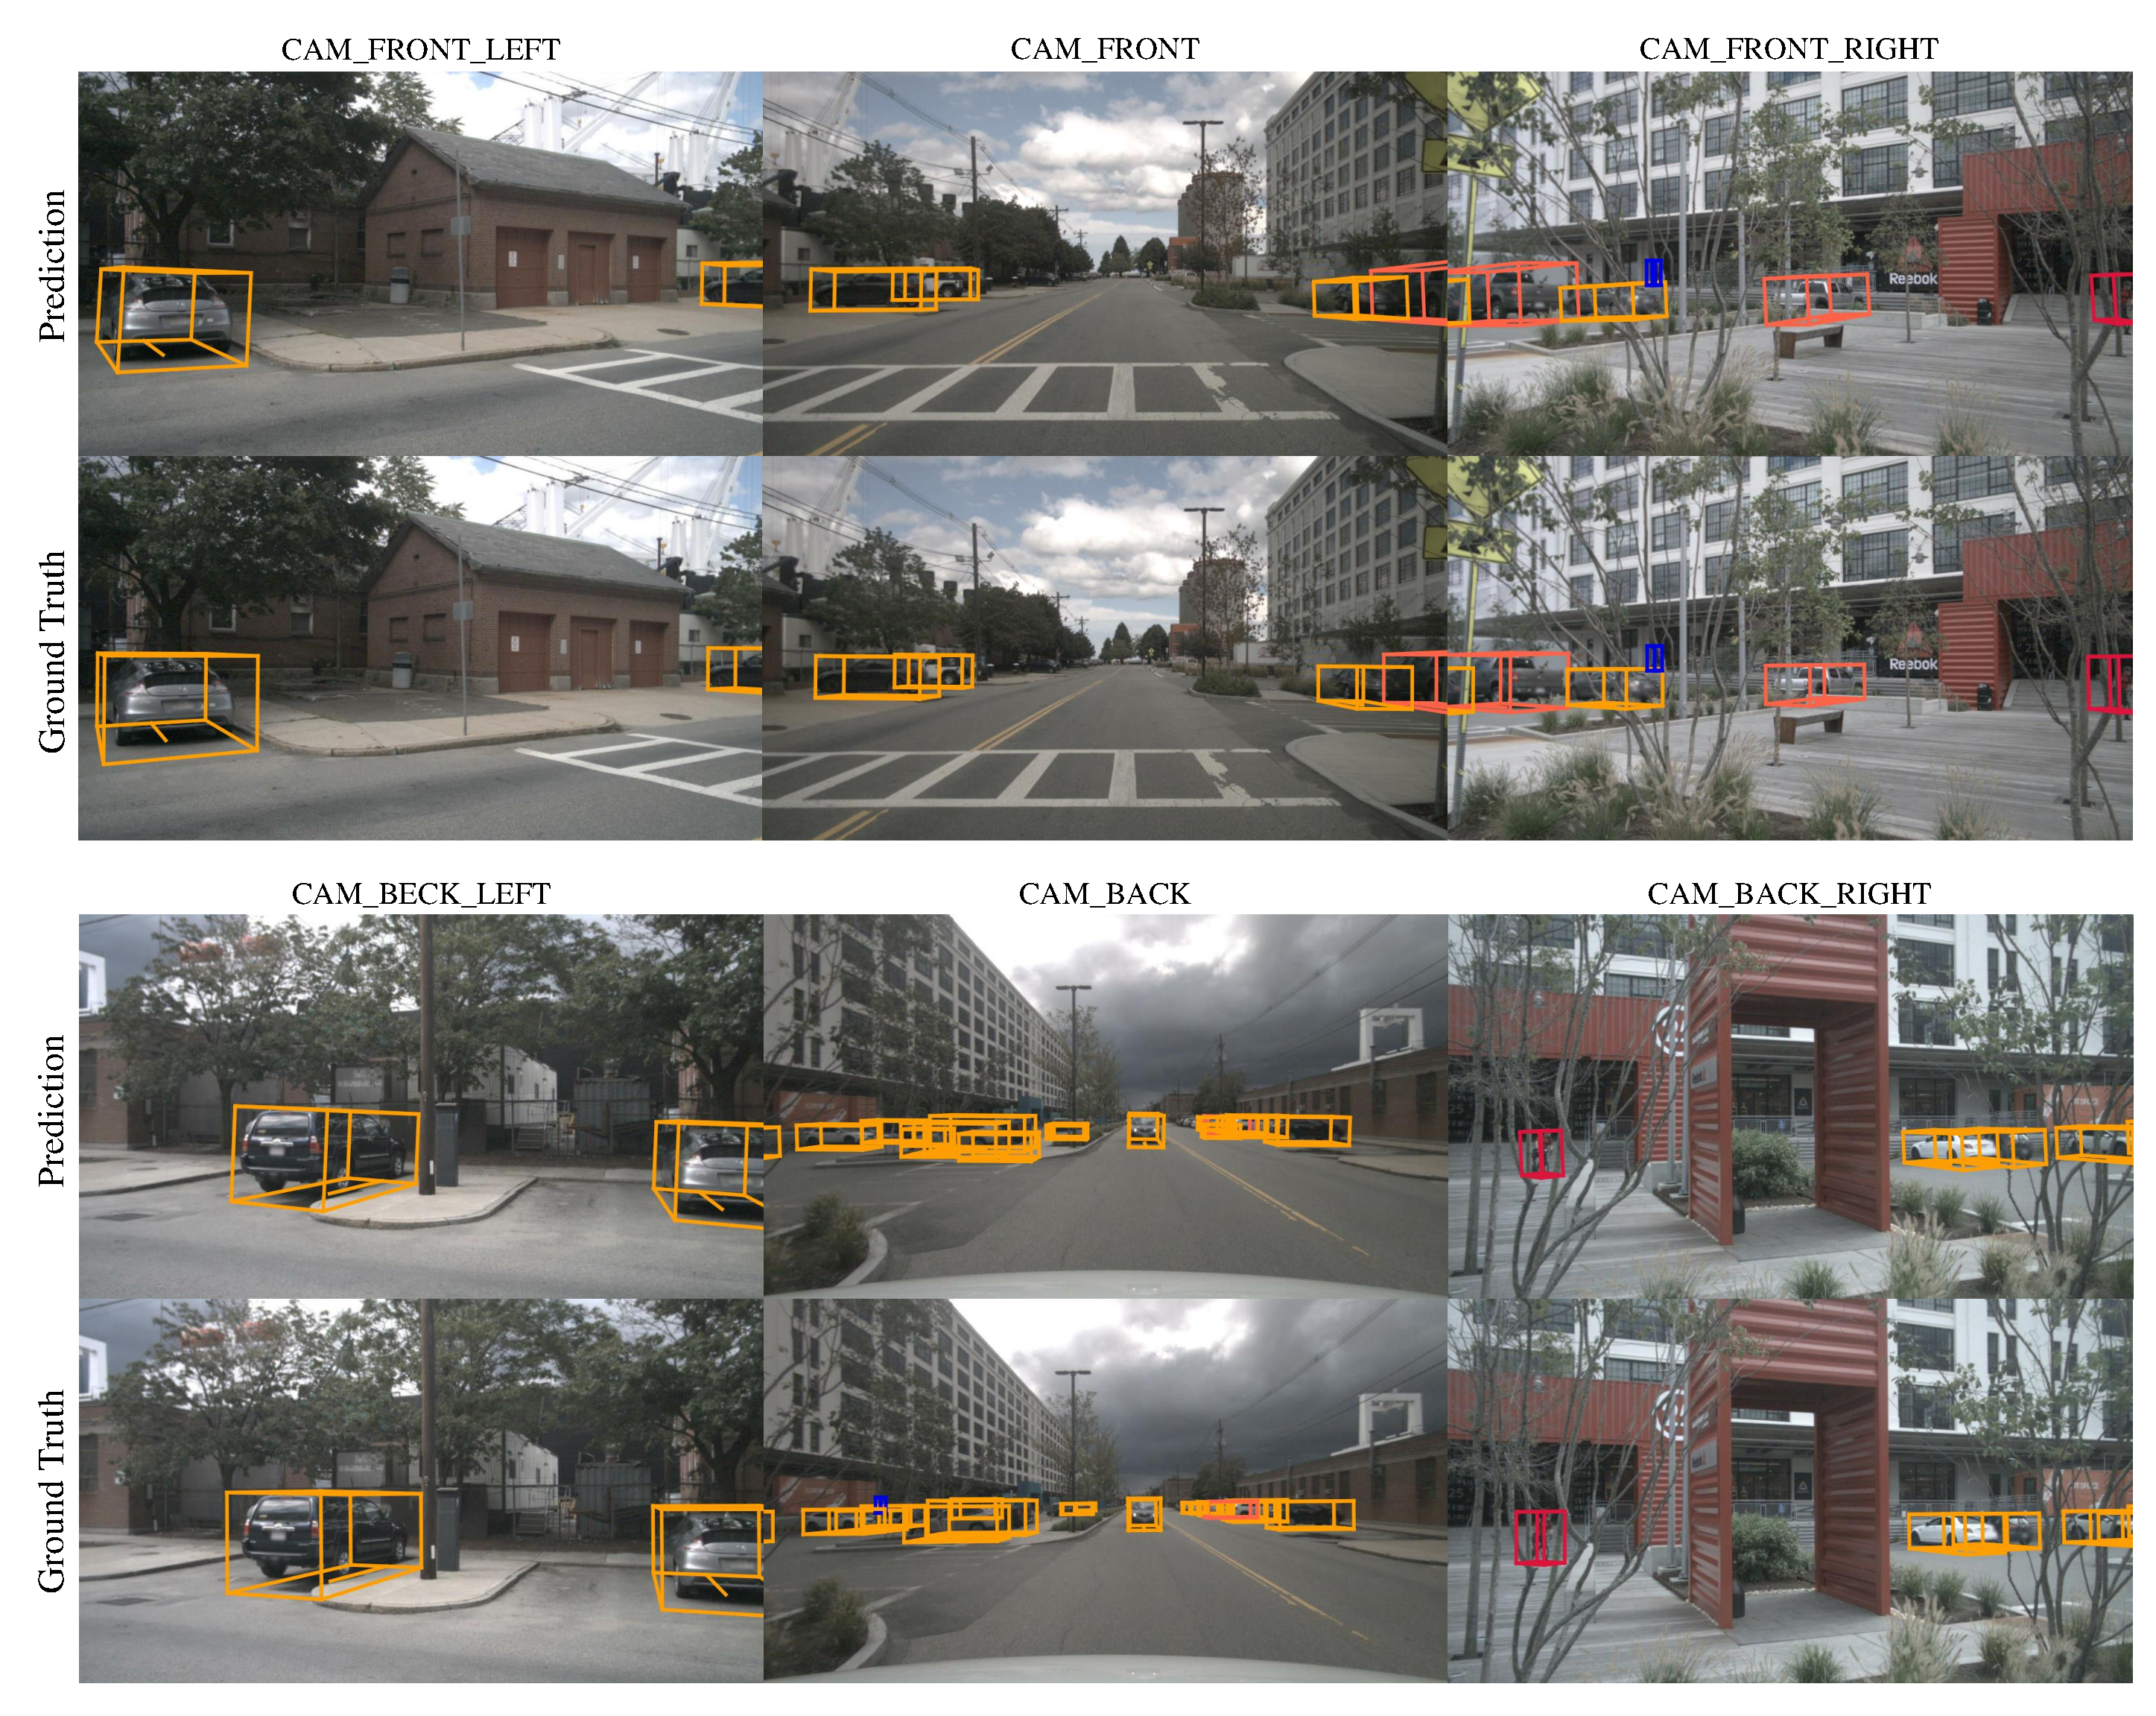
\includegraphics[width=0.8\textwidth]{figures/visualization2.pdf}
    \caption{BEVFormer v2 3D目标检测预测的可视化结果。}
    \label{fig:visualization}
\end{figure*}

\subsection{第一阶段提议的后处理}
\label{sec/appendix/post-process}
本节描述来自透视检测头的提议的后处理流程。
从透视头提供的所有相机视图的原始预测开始。
对于所有视图 $\mathcal{V}$ 中的第 $i$ 个视图，预测的3D边界框及其分数记为 $\{(\mathbf{B}_{i,j},s_{i,j})\}_j$。
通过以下后处理流程筛选出分数最高的候选。
首先，对每个视图 $i$ 的提议执行非极大值抑制（Non-maximum Suppression, NMS），以获取在透视图上无重叠的候选 $C_i$：
\begin{equation}
    C_i := \text{NMS}_{pers}\left(\{(\mathbf{B}_{i,j},s_{i,j})\}_j\right)
\end{equation}
NMS阈值设置为 2D IoU = 0.75。为确保所有相机视图中的物体都能被检测到，通过取每个视图 $i$ 在NMS后的 top-$k_1$ 来平衡不同视图的提议数量：
\begin{equation}
    C := \bigcup_{i\in\mathcal{V}} \text{top-}k_1\left(C_i\right)
\end{equation}
实验中设 $k_1=100$。
$C$ 中所有3D框通过相应的相机外参投影到鸟瞰视图坐标。
为避免出现在多个视图中的物体导致提议重叠，在BEV平面上以 BEV IoU = 0.3 应用另一个NMS：
\begin{equation}
    C := \text{NMS}_{bev}(C)
\end{equation}
最后，选择 top $k_2=100$ 个提议：
\begin{equation}
    C := \text{top-}k_2(C)
\end{equation}
对于最终提议集 $C$ 中的每个3D边界框 $\mathbf{B}$，其在BEV平面上的投影中心 $(c_x(\mathbf{B}),c_y(\mathbf{B}))$ 用作物体解码器中可变形 DETR 的参考点。


\section{可视化}
本文在 \cref{fig:visualization} 中展示了 BEVFormer v2 检测器的3D目标检测结果可视化。即使对于远处或被遮挡的困难样本，模型也能预测出准确的目标3D边界框。例如，模型成功检测到了前右相机远处的行人、后相机中与多辆车重叠的卡车，以及后右相机中被树遮挡的自行车。

% \section{进一步实证研究}
% \subsection{与深度预训练图像骨干网络的比较}
% To demonstrate that BEVFormer v2 does not require domain-specific pre-training to achieve SoTA results with large-scale image backbones, we compare BEVFormer v2 with the original BEVFormer~\cite{bevformer} using the DLA-34~\cite{DLA} and the VoVNet-99~\cite{Vovnet} backbones with different pre-training settsings in ~\cref{table:depth_pretrain}.
% \setlength{\tabcolsep}{3pt}
\setlength{\doublerulesep}{2\arrayrulewidth}
\renewcommand{\arraystretch}{1.0}
\begin{table*}[t]
    \caption{BEVFormer v2 在使用 COCO 预训练和深度预训练（Depth Pre-training）的 VoVNet-99 骨干网络时，在 nuScenes 测试集上的3D检测结果。省略 COCO 预训练的epoch数，因为 COCO 预训练骨干网络广泛可用且两种设置使用相同的 COCO 预训练。}
    \label{table:depth_pretrain}
    \centering

    \begin{tabular}{c|c|c|cc|cccccc}
        \toprule
        Backbone & Epoch & Pre-train & NDS & mAP & mATE & mASE & mAOE & mAVE & mAAE   \\ 
        \midrule
        DLA-34 & 72 & COCO & & & & & & & & \\ 
        DLA-34 & \small{15M Img + 120 + 24} & \small{COCO $\xrightarrow{}$ DDAD15M $\xrightarrow{}$ nuScenes} & & & & & & & \\ 
        \midrule
        VoVNet-99 & 72 & COCO & & & & & & & & \\ 
        VoVNet-99 & \small{15M Img + 120 + 24} & \small{COCO $\xrightarrow{}$ DDAD15M $\xrightarrow{}$ nuScenes} & & & & & & & \\ 
        \bottomrule
    \end{tabular}
\end{table*}

% \subsection{大规模图像骨干网络在长训练计划下的性能}
% \setlength{\tabcolsep}{3pt}
\setlength{\doublerulesep}{2\arrayrulewidth}
\renewcommand{\arraystretch}{1.0}
\begin{table*}[ht]
    \caption{InternImage-XL 在延长训练计划下，在 nuScenes 测试集上的3D检测结果。}
    \label{table:extend_training}
    \centering

    \begin{tabular}{c|c|cc|cccccc}
        \toprule
        Backbone & Epoch & NDS & mAP & mATE & mASE & mAOE & mAVE & mAAE   \\ 
        \midrule
        InternImage-XL & 24 & & & & & & & \\ 
        InternImage-XL & 48 & & & & & & & \\ 
        InternImage-XL & 72 & & & & & & & \\ 
        \bottomrule
    \end{tabular}
    
\end{table*}
